\documentclass[11pt]{report}



\usepackage{wrapfig, graphicx}





\usepackage[total={5.9in,8.86in},top=1.2in, includefoot]{geometry}
\usepackage[font={small},labelfont=bf, justification=raggedright]{caption}
\usepackage{subfig}
\newcommand{\credit}[1]{\textit{(Photo: #1)}}
\setcounter{secnumdepth}{3}

\begin{document}



\begin{titlepage}
 \begin{center}

\textsc{\large University of Toronto}\\[1.1cm]
\textsc{\normalsize AER201, January 2010}\\[1.5cm]

% Title

{ \huge \bfseries Helical Cone Deployment Machine}\\[2.4cm]

% and supervisor
\begin{minipage}{0.4\textwidth}
\begin{flushleft} \large
\emph{Author:}\\
Ahil Ganesh (997xxxxxx)\\
Sebastian Kosch (997241024)\\
Karl Qin (997xxxxxx)\\
\end{flushleft}
\end{minipage}
\begin{minipage}{0.4\textwidth}
\begin{flushright} \large
\emph{Supervisor:} \\
Dr. Reza Emami
\end{flushright}
\end{minipage}

\vfill

% Bottom of the page
{\large \today}

\end{center}
\end{titlepage}

\chapter{Executive Summary}


\chapter{Introduction}

\section{Statement of Need}

We \textit{really} need these, because traffic workers die all the time.

\section{Goals and Objectives}

\section{Background Research}

\subsection{Existing Designs}

\begin{figure}
  \centering
  \subfloat[Autocone]{\label{fig:gull}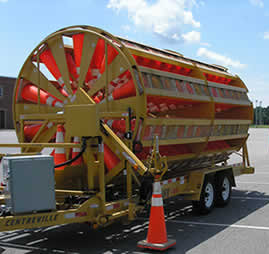
\includegraphics[width=0.45\textwidth]{autocone}}\hspace{20pt}                
  \subfloat[TRAF-tech ACM]{\label{fig:tiger}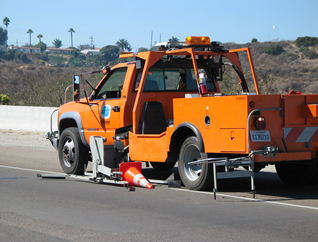
\includegraphics[width=0.45\textwidth]{traftech}}
   \caption{Existing designs \credit{http://www.innovativequip.com/, http://www.traftech.net/}}
  \label{fig:exisitingdesigns}
\end{figure}

\subsubsection{Autocone}
The Autocone 130 is a large trailer that stores up to 130 traffic cones. It uses a hydraulic system both to deploy the cones and to pick up cones standing or lying on the road. The cones are stored in a revolving framework. Within the framework, the cones are moved to the deployment arm by means of a chain conveyor system \cite{HowItsMade-Autocone}. While the compactness of the revolving frame is convincing, the capacity is far higher than that required in this project. For this prototype, designing an intricate miniature hydraulic arm is thus not justifiable.

\subsubsection{TRAF-tech ACT/M Series}
TRAF-tech commercialized the cone deployment system initially developed by the California Department of Transportation. Two different implementations are available: one uses rails to deploy the cones, the other a hydraulic arm. Both rely on belt systems to move the individual cones from the stack to the deployment mechanism. Like Autocone, TRAF-tech offers systems with a comparatively high cone capacity. Conveyor belts, however, are difficult to build reliably,\footnote{as has been confirmed by past AER201 students.} and may not be of much help with the more flexible toy cones at hand.


\subsection{Possible solutions for the given RFP}


\chapter{Technical Body}

\section{Statement of Work}
\subsection{Components}
\subsubsection{Mechanical}
\paragraph{Wheels}
The wheels are ...
\paragraph{Coils}
The coils move the cones.
\subsubsection{Electronic/Sensors}
\paragraph{Driver Board}
Made by Karl, this customized driver board is awesome.
\paragraph{Sensors}
Special sensors.
\subsubsection{Microcontroller}
A single microcontroller processes the sensors' inputs, computes the power delivered to the motors, and interacts with the user via a matrix keypad and a 16$\times$2 character LCD. 
\paragraph{Choice of model}
The microcontroller used is a 40-pin PIC chip by Microchip, model 18F4620. The model was chosen over model 16F877, which was given with the development board, mainly for its interrupt capabilities. The 16F series provides an external interrupt channel on pin \texttt{RB0}. Unfortunately, this does not allow for interrupt-based development with the development board's keypad, since the keypad's \texttt{DataReady}-flag is hardwired to \texttt{RB1}. Using the Interrupt-on-change feature on \texttt{RB4:7} does not help; pressing the same key twice will not raise an interrupt. The same rationale explains the choice of a 40-pin model. While all functionality could have been implemented, tested and debugged on the development board with the given 16F877 series PIC, interrupt-based code is easier to debug than code littered with \texttt{goto}-based polling points.  

\paragraph{Program flow and menu}
On power-on, the microcontroller initializes memory, interrupt bits and I/O settings. It then waits for input on interrupt lines. [SOMETHING ABOUT POWER CONSUMPTION IN THE LOOP VS. POLLING]. The following events should raise an interrupt:
\begin{itemize}
  \item{the user presses a key on the keypad,}
  \item{the interval timer overflows to cause a cone to be deployed,}
  \item{the reflection sensor reports a hole,}
  \item{all cones have been deployed, or a distance of 3 meters was covered,}
  \item{the side reflection sensors report crossing the lane.}
\end{itemize}
\begin{figure}
  \centering
  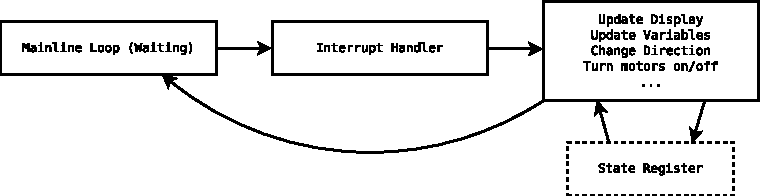
\includegraphics{program_flow.pdf}
  \caption{General flow of the microcontroller program}
  \label{fig:programflow}
\end{figure}
The interrupt service routine (ISR) will then determine the type of interrupt. A state register holds a numerical value representing the current state of the device, such as \textit{Menu, Screen 3} or \textit{Returning from deployment}. Depending on the current state, the ISR calls subroutines to handle the input. Example: during user interaction, this might mean storing the input and updating the display; during deployment, this might mean rotating the coil or decelerating the motors. It may also include changing the state register. Eventually, all subroutines will return to the \texttt{Mainline} loop to save power.

\subsection{Functional Description}
The cone deployment machine will prompt the user for input, deploy the cones, return to the user and display information about the deployment. This communication happens via a 4$\times$4 matrix keypad (keys 0--9 and A--D) and a 16$\times$2 character LCD with standard HD44780 interface. To make operation as easy as possible, the interaction using display and keypad should be self-explanatory to the user. Therefore, we designed a near-linear sequence of inputs and outputs that leads the user through all necessary steps. This is adequate for both novices and experiences users. Figure \ref{fig:menuflow} provides an overview.

The machine will go and dispense cones. ... bla.



\subsection{Evaluation Plan}
\subsubsection{Process evaluation}

\subsubsection{Product evaluation}


\section{Schedule}
Bar chart, bar chart, bar chart.

\section{Budget}


\chapter{Conclusion}


\appendix
\chapter{Appendix}
\section{Figures and Tables}
\begin{figure}
  \centering
  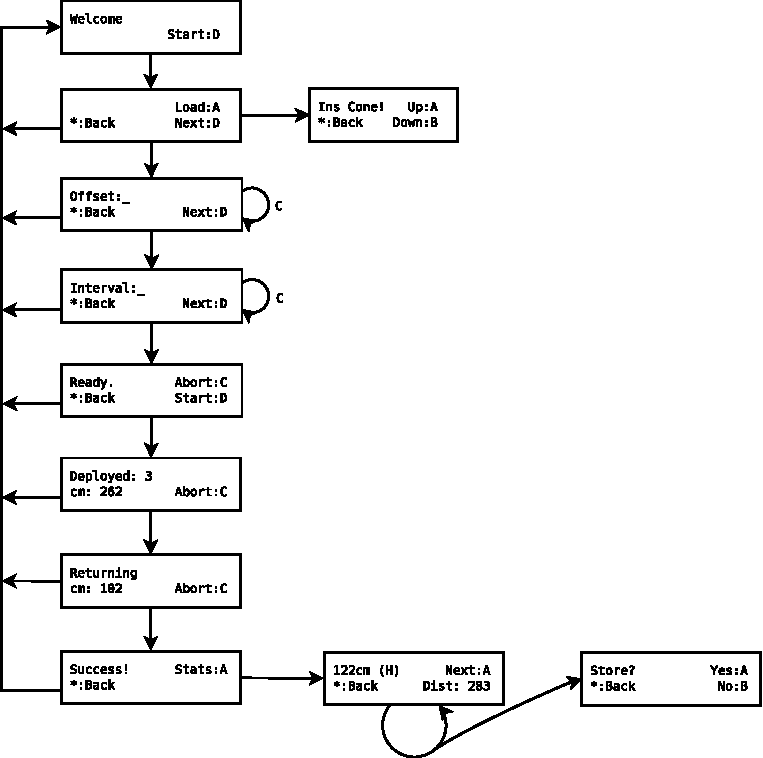
\includegraphics{menu_flowchart.pdf}
  \caption{Sequence of menu displays navigable by the user}
  \label{fig:menuflow}
\end{figure}

%\bibliography{


%}

\end{document}
